  \let\negmedspace\undefined
\let\negthickspace\undefined
\documentclass[journal]{IEEEtran}
\usepackage[a5paper, margin=10mm, onecolumn]{geometry}
\usepackage{lmodern} % Ensure lmodern is loaded for pdflatex
\usepackage{tfrupee} % Include tfrupee package

\setlength{\headheight}{1cm} % Set the height of the header box
\setlength{\headsep}{0mm}     % Set the distance between the header box and the top of the text

\usepackage{gvv-book}
\usepackage{gvv}
\usepackage{cite}
\usepackage{amsmath,amssymb,amsfonts,amsthm}
\usepackage{algorithmic}
\usepackage{graphicx}
\usepackage{textcomp}
\usepackage{xcolor}
\usepackage{txfonts}
\usepackage{listings}
\usepackage{enumitem}
\usepackage{mathtools}
\usepackage{gensymb}
\usepackage{comment}
\usepackage[breaklinks=true]{hyperref}
\usepackage{tkz-euclide} 
\usepackage{listings}                                      
\def\inputGnumericTable{}                                 
\usepackage[latin1]{inputenc}                                
\usepackage{color}                                            
\usepackage{array}                                            
\usepackage{longtable}
\usepackage{multicol}
\usepackage{calc}                                             
\usepackage{multirow}                                         
\usepackage{hhline}                                           
\usepackage{ifthen}                                           
\usepackage{lscape}
\begin{document}

\bibliographystyle{IEEEtran}
\vspace{3cm}

\title{1.1.2.2}
\author{EE24BTECH11024 - G. Abhimanyu Koushik}
% \maketitle
% \newpage
% \bigskip
{\let\newpage\relax\maketitle}

\renewcommand{\thefigure}{\theenumi}
\renewcommand{\thetable}{\theenumi}
\setlength{\intextsep}{10pt} % Space between text and floats


\numberwithin{equation}{enumi}
\numberwithin{figure}{enumi}
\renewcommand{\thetable}{\theenumi}


\textbf{Question}:\newline
Find the values of $x,y,z$ so that the vectors $x\hat{i}+2\hat{j}+z\hat{k}$ and $2\hat{i}+y\hat{j}+\hat{k}$ are equal
\newline
\textbf{Solution: }
\begin{table}[h!]    
  \centering
  \begin{tabular}[12pt]{ |c|c|c|}
    \hline
    \textbf{Symbol} & \textbf{Value} & \textbf{Description} \\
    \hline
    $\vec{A}$ & \myvec{6\\5} & First point\\
    \hline 
    $\vec{B}$ & \myvec{-4\\3} & Second point\\
    \hline
    $\vec{Y}$ & \myvec{0\\$y$} & Point on Y-Axis equidistant from A and B\\
    \hline
    \end{tabular}

  \caption{Variables Used}
  \label{tab1.1.2.2}
\end{table}
\newline
If the vectors are equal then the vector component along the X,Y and Z axes should also be equal
\begin{align}
\overrightarrow{v}_1\cdot \hat{i} &= \overrightarrow{v}_2\cdot \hat{i}\\
\brak{x\hat{i}+2\hat{j}+z\hat{k}} \cdot \hat{i} &= \brak{2\hat{i}+y\hat{j}+\hat{k}} \cdot \hat{i}\\
x\times 1+2\times 0+ z\times 0&=2\times 1+y\times 0+ 1\times 0\\
x+0+0&=2+0+0\\
x&=2
\end{align}
Similarly, taking dot product with $\hat{j}$ and $\hat{k}$ will give the values of $y$ and $z$.\\
Dot product with $\hat{j}$
\begin{align}
\overrightarrow{v}_1\cdot \hat{j} &= \overrightarrow{v}_2\cdot \hat{j}\\
\brak{x\hat{i}+2\hat{j}+z\hat{k}} \cdot \hat{j} &= \brak{2\hat{i}+y\hat{j}+\hat{k}} \cdot \hat{j}\\
x\times 0+2\times 1+ z\times 0&=2\times 0+y\times 1+ 1\times 0\\
0+2+0&=0+y+0\\
y&=2
\end{align}
Dot product with $\hat{k}$
\begin{align}
\overrightarrow{v}_1\cdot \hat{k} &= \overrightarrow{v}_2\cdot \hat{k}\\
\brak{x\hat{i}+2\hat{j}+z\hat{k}} \cdot \hat{k} &= \brak{2\hat{i}+y\hat{j}+\hat{k}} \cdot \hat{k}\\
x\times 0+2\times 0+ z\times 1&=2\times 0+y\times 0+ 1\times 1\\
0+0+z&=0+0+1\\
z&=1
\end{align}
The values of $x,y,z$ are $2,2,1$ respectively.
\begin{figure}[h!]
   \centering
   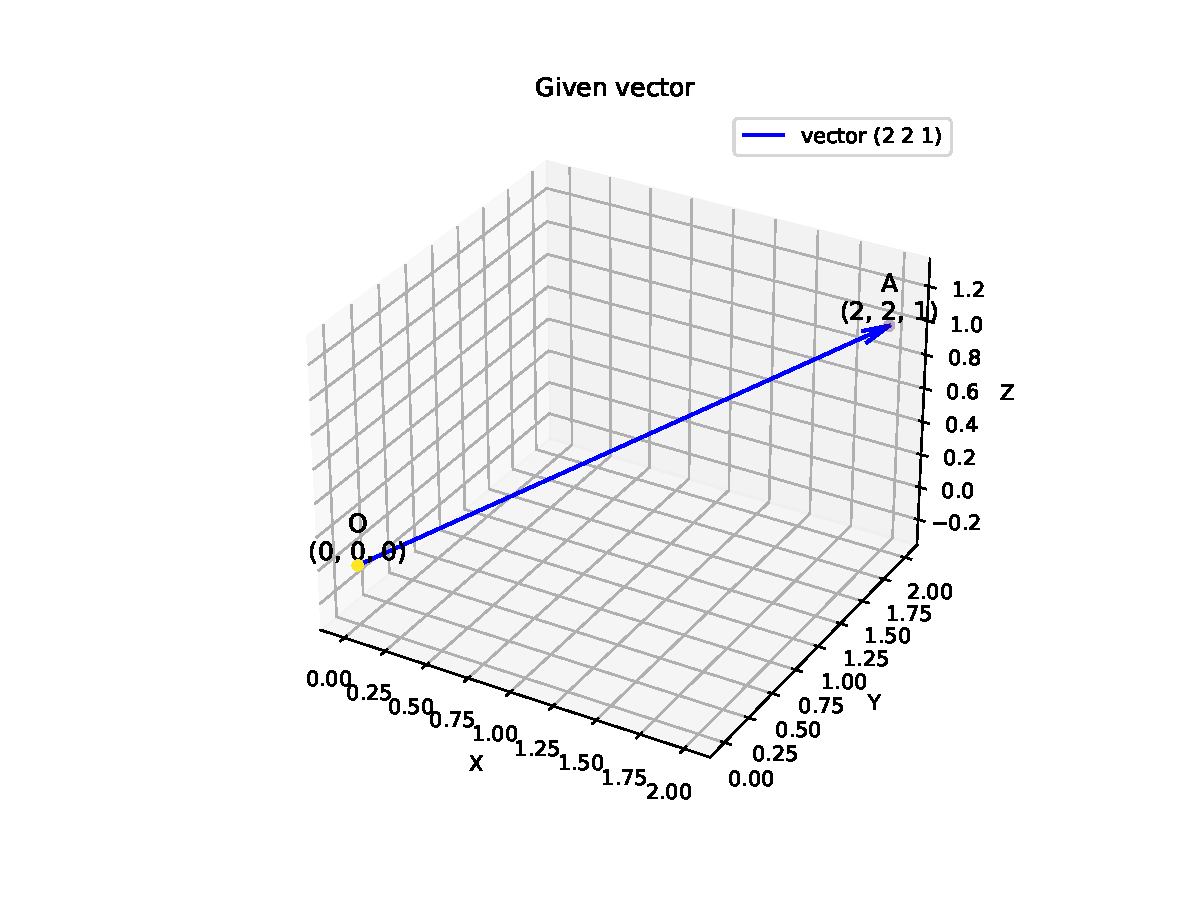
\includegraphics[width=1\linewidth]{figs/fig.pdf}
   \caption{Line segment represent the vector}
   \label{stemplot}
\end{figure}
\end{document}  
\end{document}


